\chapter{Thuật toán A*}
\ifpdf
    \graphicspath{{Chapter2/Chapter2Figs/PNG/}{Chapter2/Chapter2Figs/PDF/}{Chapter2/Chapter2Figs/}}
\else
    \graphicspath{{Chapter2/Chapter2Figs/EPS/}{Chapter2/Chapter2Figs/}}
\fi

\section{Giới thiệu thuật toán}
Trong khoa học máy tính, A* (đọc là A sao) là thuật toán tìm kiếm trong đồ thị. Thuật toán này tìm một đường đi từ một nút khởi đầu tới một nút đích cho trước (hoặc tới một nút thỏa mãn một điều kiện đích). Thuật toán này sử dụng một "đánh giá heuristic" để xếp loại từng nút theo ước lượng về tuyến đường tốt nhất đi qua nút đó. Thuật toán này duyệt các nút theo thứ tự của đánh giá heuristic này. Do đó, thuật toán A* là một ví dụ của tìm kiếm theo lựa chọn tốt nhất (best-first search).\\

Thuật toán A* được mô tả lần đầu vào năm 1968 bởi Peter Hart, Nils Nilsson, và Bertram Raphael. Trong bài báo của họ, thuật toán được gọi là thuật toán A; khi sử dụng thuật toán này với một đánh giá heuristic thích hợp sẽ thu được hoạt động tối ưu, do đó mà có tên A*.\\

Năm 1964, Nils Nilsson phát minh ra một phương pháp tiếp cận dựa trên khám phá để tăng tốc độ của thuật toán Dijkstra. Thuật toán này được gọi là A1. Năm 1967 Bertram Raphael đã cải thiện đáng kể thuật toán này, nhưng không thể hiển thị tối ưu. Ông gọi thuật toán này là A2. Sau đó, trong năm 1968 Peter E. Hart đã giới thiệu một đối số chứng minh A2 là tối ưu khi sử dụng thuật toán này với một đánh giá heuristic thích hợp sẽ thu được hoạt động tối ưu. Chứng minh của ông về thuật toán cũng bao gồm một phần cho thấy rằng các thuật toán A2 mới là thuật toán tốt nhất có thể được đưa ra các điều kiện. Do đó ông đặt tên cho thuật toán mới là A *(A sao, A-star).\\

Trong khoa học máy tính, A* thuật toán tìm kiếm trong đồ thị. Thuật toán này tìm một đường đi từ nút khởi đầu đến nút đích dựa trên cách đánh giá Heuristic để tìm ra con đường tốt nhất cho thuật toán. Điểm khác biệt của A* đối với tìm kiếm theo lựa chọn tốt nhất là nó còn tính khoảng cách đã đi qua. Điều này làm cho A* đầy đủ và tối ưu, nghĩa là với thuật toán này sẽ luonon tìm thấy đường đi ngắn nhất nếu tồn tại.\\

\section{Hàm ước lượng Heuristic}
Heuristic là phương pháp giải quyết vấn đề dựa trên phỏng đoán, ước chừng, kinh nghiệm, trực giác để tìm ra giải pháp gần như là tốt nhất và nhanh chóng.\\
Hàm Heuristic là hàm ứng với mỗi trạng thái hay mỗi sự lựa chọn một giá trị ý nghĩa đối với vấn đề dựa vào giá trị hàm này ta lựa chọn hành động.

\section{Mô tả thuật toán}
 Giả sử n0 là trạng ban đầu và n là trạng thái hiện tại, ta có đường đi từ n0 đến n được xác định bằng hàm: f(n) = g(n) + h(n). Trong đó:\\
1/ g(n) là chi phí từ nút gốc đến nút hiện tại n.\\
2/ h(n) chi phí ước lượng từ nút hiện tại n tới đích.\\
3/ f(n) chi phí tổng của n0 đến n.\\

Đường đi được xem là chấp nhận được nếu với mọi nút ở trạng thái n: 0 <= h(n) <=h*(n).\\
Trong đó h*(n) là chi phí thực tế để hoàn thành bài toán.\\

Áp dụng vào bài toán 8 Puzzle như sau:\\
Đầu vào: trạng thái ban đầu và trạng thái đích.\\
Đầu ra: tập dữ liệu tất cả các trạng thái từ trạng thái ban đầu đến trạng thái đích.\\
Điều kiện dừng thuật toán: tìm thấy kết quả trạng thái trùng với trạng thái đích.\\

Thực hiện bài toán: \\
B1: Thực hiện tính toán các vị trí sai của trạng thái hiện tại so với trạng thái đích và tính chi phí theo công thức f(n) = g(n) + h(n) để chọn ra đường đi tốt nhất. \\
B2: Tiến hành di chuyển vị trí 1 trong các còn sai vị trí và lặp lại bước số 1 cho đến khi tìm ra kết quả. Lưu ý trạng thái đạt được phải khác với trạng thái của những lần thực hiện trước đó.\\

Dưới đây là hình minh họa cho quá trình thực hiện bài toán\\

\begin{figure}[!htbp]
  \begin{center}
    \leavevmode
    \ifpdf
      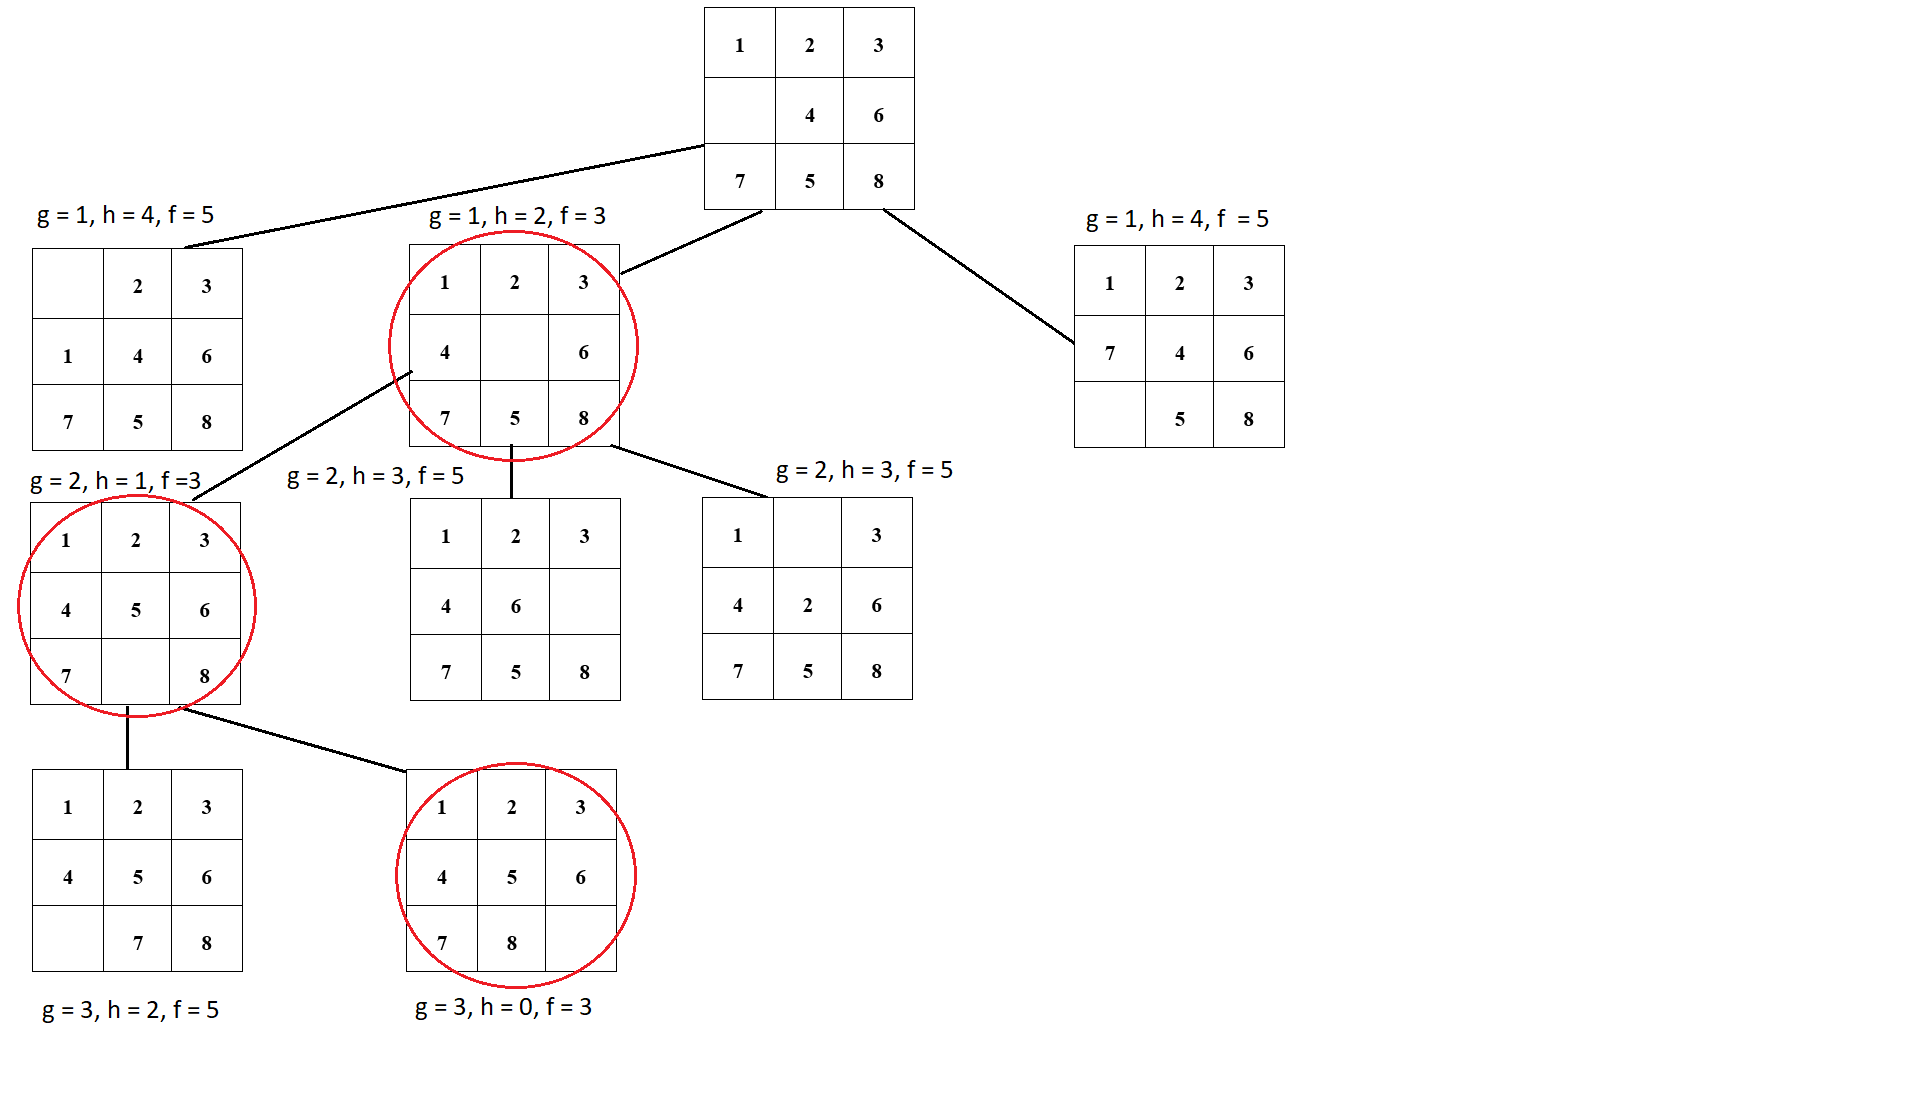
\includegraphics[height=5in]{Flow}
    \else
      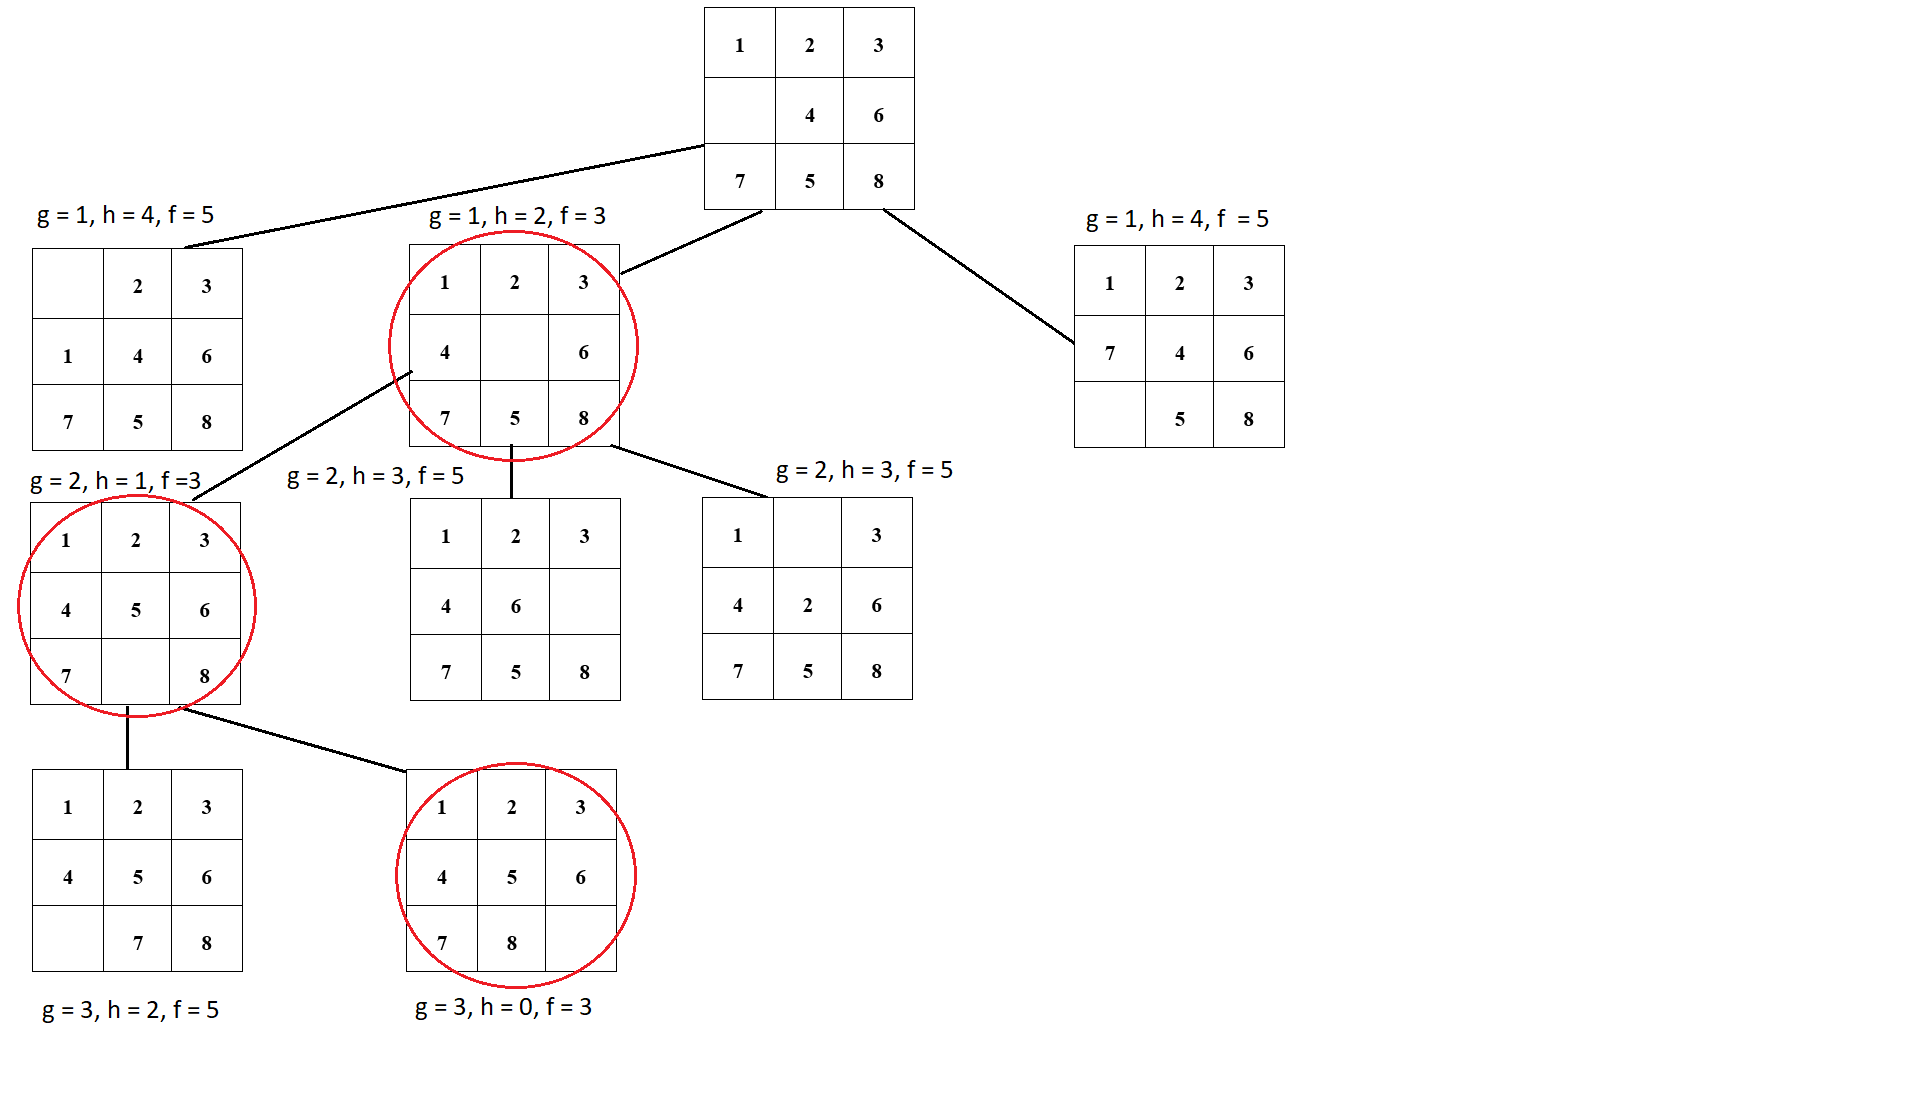
\includegraphics[bb = 92 86 545 742, height=5in]{Flow}
    \fi
    \caption{Khởi tạo Class}
    \label{FigAir}
   
  \end{center}
\end{figure}
\FloatBarrier



\section{Áp dụng thuật toán A* vào bài toán sử dụng C++}
\subsection{Khởi tạo Class và Function}
Cài đặt thuật toán A* bài toán ta dùng một Class puzzleArray. Class này gồm 1 mảng 2 chiều 3x3 và các thông số khác bao gồm: \\
1/ Vị trí x,y nhằm xác định vị trí phần tử của mảng puzzleArray, trong đó phần tử giá trị 0 là đại diện cho ô trống trên Puzzle.\\
2/ canMove thể hiện phần tử có thể duy chuyển sang vị trí mới hay không.\\
3/ Check \\
5/ Cost là chi phí tối đa để thực hiện cho bài toán này.\\
Bên cạnh đó, class puzzleArray còn có những Function sau:\\
1/ checkCost: trả về chi phí dự tính f(n).\\
2/ checkMoveLeft, checkMoveRight, checkMoveUp, checkMoveDown để xác định hướng mà phần tử có thể di chuyển.\\
3/ moveLeft, moveRight, moveUp, moveDown: hàm thực hiện đổi chỗ các phần tử liền kề với nhau.\\
4/ checkFinish: kiểm tra mảng đã trùng với trạng thái đích hay chưa. Nếu trùng thì bài toán sẽ kết thúc.
\begin{figure}[!htbp]
  \begin{center}
    \leavevmode
    \ifpdf
      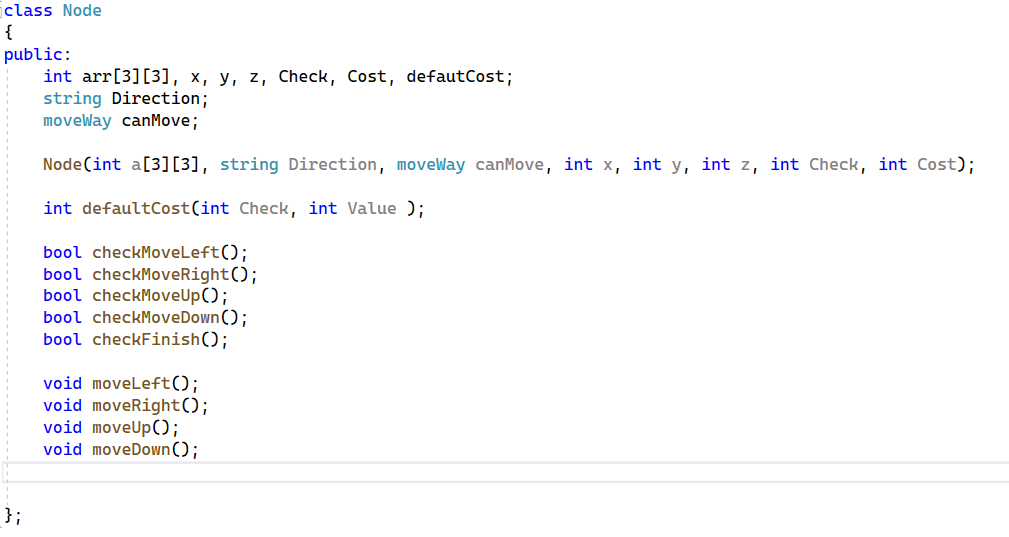
\includegraphics[height=3in]{ClassNode}
    \else
      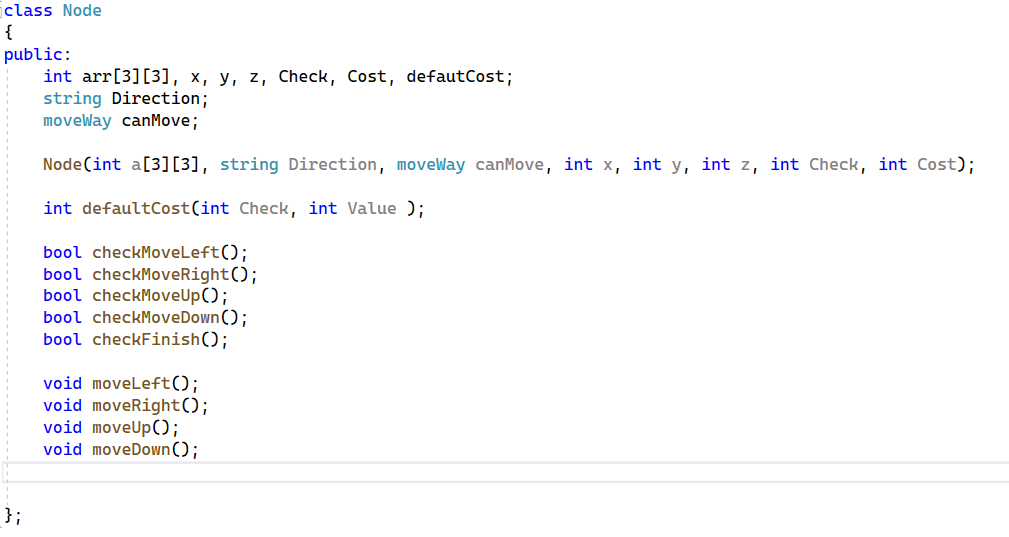
\includegraphics[bb = 92 86 545 742, height=3in]{ClassNode}
    \fi
    \caption{Mô tả quá trình thực hiện bài toán}
    \label{FigAir}
   
  \end{center}
\end{figure}
\FloatBarrier

\subsection{Một số hàm liên quan trong thuật toán}
Hàm kiểm tra phần tử trong mảng có thể di chuyển hay không.\\
\begin{figure}[!htbp]
  \begin{center}
    \leavevmode
    \ifpdf
      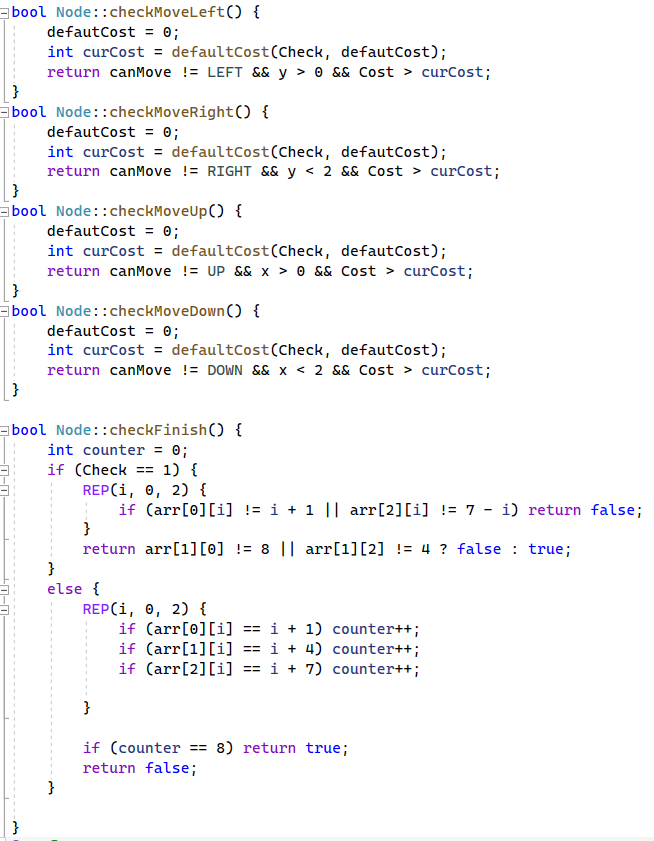
\includegraphics[height=6in]{CheckMove}
    \else
      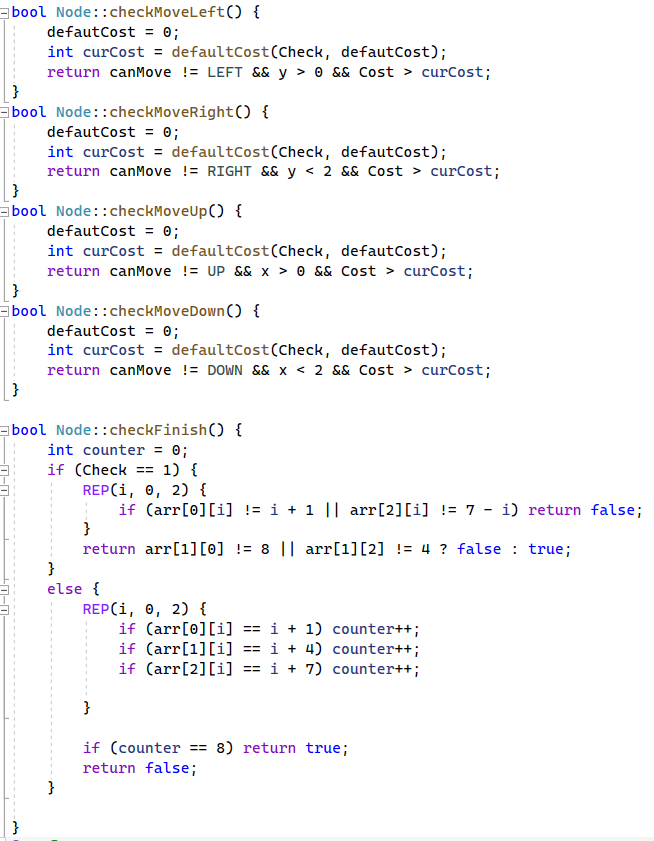
\includegraphics[bb = 92 86 545 742, height=6in]{CheckMove}
    \fi
    \caption{Một số hàm kiểm tra}
    \label{FigAir}
   
  \end{center}
\end{figure}
\FloatBarrier
Hàm di chuyển.\\
\begin{figure}[!htbp]
  \begin{center}
    \leavevmode
    \ifpdf
      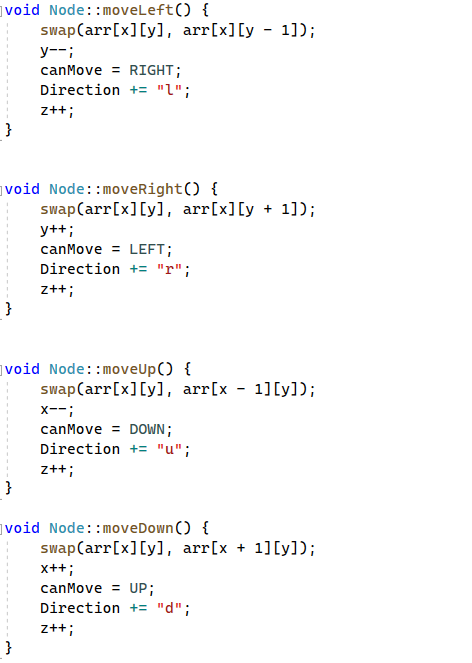
\includegraphics[height=6in]{Move}
    \else
      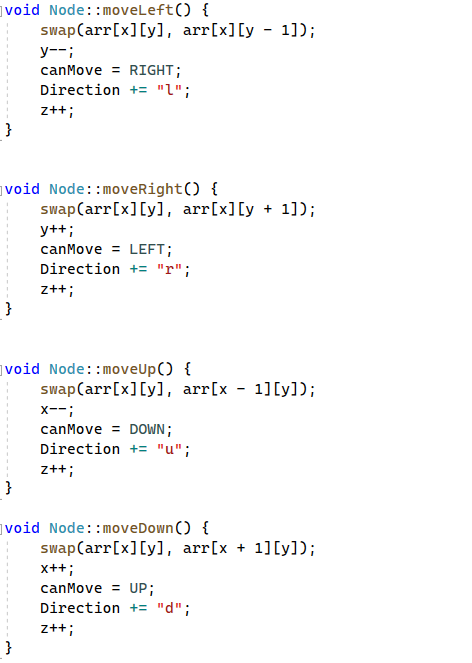
\includegraphics[bb = 92 86 545 742, height=6in]{Move}
    \fi
    \caption{Hàm di chuyển}
    \label{FigAir}
   
  \end{center}
\end{figure}
\FloatBarrier
\subsection{Kết quả đạt được}
Kết quả đạt được sau khi chạy thuật toán.\\
\begin{figure}[!htbp]
  \begin{center}
    \leavevmode
    \ifpdf
      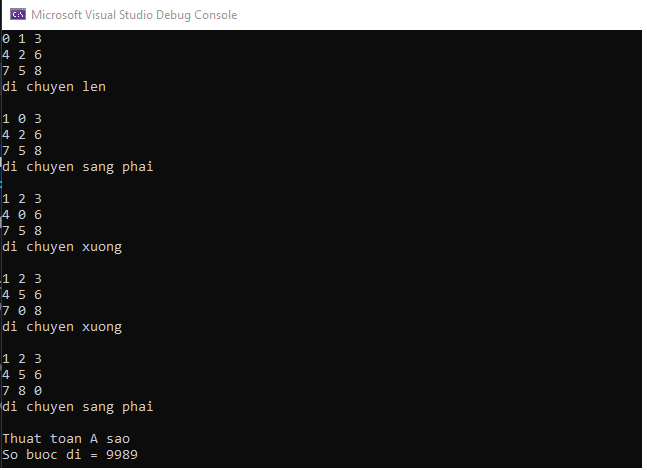
\includegraphics[height=4in]{Result}
    \else
      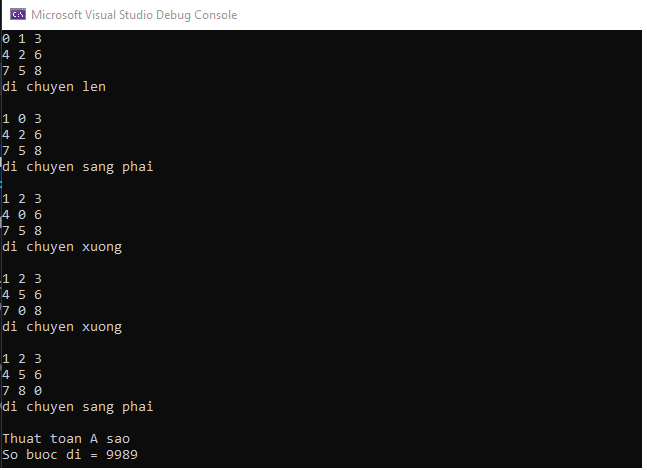
\includegraphics[bb = 92 86 545 742, height=4in]{Result}
    \fi
    \caption{Một số hàm kiểm tra}
    \label{FigAir}
   
  \end{center}
\end{figure}
\FloatBarrier

